\documentclass[prd,preprintnumbers,floatfix,
nofootinbib,superscriptaddress]{revtex4}

%------------------

\usepackage{float}
\usepackage{nicefrac}
\usepackage{mathtools}
\usepackage{amsfonts}
\usepackage{amssymb}
\usepackage{amsmath}
\usepackage{graphicx}
\usepackage{subfigure}
\usepackage{array}
\usepackage{dcolumn}
\usepackage{bm}
\usepackage{esint}
\usepackage{xcolor}
\usepackage{longtable} % long tables
\usepackage{hyperref}
\usepackage{verbatim}
\usepackage{epsfig}
\usepackage{slashed}
\usepackage{color}


\newcommand{\diff}{\mathrm{d}}
\newcommand{\ket}[1]{\ensuremath{\left|#1\right\rangle}}
\newcommand{\bra}[1]{\ensuremath{\left\langle #1\right|}}
\newcommand{\TS}{\mathrm{TS}}
\newcommand{\LLH}{\mathrm{LLH}}
\newcommand{\M}{\mathcal{M}}
%
\newcommand{\I}{\ensuremath{I}}
\newcommand{\II}{\ensuremath{{I\!I}}}
\newcommand{\III}{\ensuremath{{I\!I\!I}}}
\newcommand{\IV}{\ensuremath{{I\!V}}}

\begin{document}
\title{Decay to two identical vectors, revisited.}

%%%%%%%%%%
\author{Mikhail Mikhasenko}
\email[e-mail: ]{mikhail.mikhasenko@cern.ch}
\affiliation{CERN-EP, CH-1211, Geneva, Switzerland}
%%%%%%%%%%

%%%%%%%%%%
\date{\today}
%%%%%%%%%%

%%%%%%%%%%
\begin{abstract}
The document presents exploratory studies of $J/\psi (\mu^+\mu^-)\,J/\psi (\mu^+\mu^-)$ system,
we well as $\phi (K^+K^-)\,\phi (K^+K^-)$.
It can be used for determination of the Higgs-boson spin.
Model-independent approach relying on rotational symmetries.
\end{abstract}
%%%%%%%%%%

\nopagebreak
\maketitle

\definecolor{cola}{rgb}{0.9,0.62,0.0}
\definecolor{colb}{rgb}{0.337, 0.706, 0.914 }
\definecolor{colc}{rgb}{0.0, 0.62, 0.451}
%
\section{Introduction}

Model-independent analysis of the particle interaction based on the
symmetries requires~\cite{Jacob:1959at}.

The Landau-Yang theorem~\cite{Yang:1950rg,Landau:1948kw}
Previous analysis of the $H\to VV$ decay~\cite{Treiman:1978ge}.
% Observation of the key $\phi$ dependence (Yang's parity test)~\cite{}.

General consideration of lepton angular distribution~\cite{Collins:1977iv}.

Extensive phenomenological analysis of four-lepton production at LHC~\cite{Bolognesi:2012mm,Gao:2010qx}

Higgs to 4l analysis~\cite{Aad:2013xqa,CMS:2018mmw}

\section{Angular amplitude}

\begin{figure}
  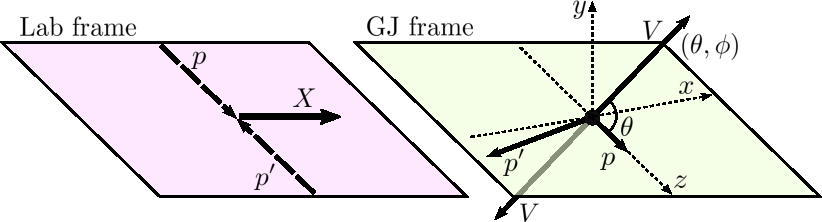
\includegraphics[width=0.6\textwidth]{../plots/production_GJ.pdf}
  \caption{Schematic view of kinematics of $X$ state produced at the $pp$ collider and decaying to two identical particles denoted by $V$. The black arrows shows three dimensional vectors of particles. A shaped arrow gives the direction of polarization of $X$.
  % The dashed lines
  }
  \label{fig:production}
\end{figure}
The measured intensity
\begin{align}
    I(\theta,\theta_1,\phi_1,\theta_2,\phi_2) &= \sum_{M}P_M
    \sum_{\xi_1,\xi_2}^{\{-1,1\}}
    \left|A^{M}_{\xi_1,\xi_2}(\theta,\theta_1,\phi_1,\theta_2,\phi_2)\right|^2,
\end{align}
where the production amplitude is given by
\begin{align}
  A^{M}_{\xi_1,\xi_2}(\theta,\theta_1,\phi_1,\theta_2,\phi_2) &= 3
  \sum_{\lambda_1,\lambda_2}
  d_{M,\lambda_1-\lambda_2}^{J}(\theta) (-1)^{1-\lambda_2}
  H_{\lambda_1\lambda_2}
  e^{i\lambda_1\phi_1+i\lambda_2\phi_2}
  d_{\lambda_1,\xi_1}^{1}(\theta_1) d_{\lambda_2,\xi_2}^{1}(\theta_2).
\end{align}
The helicity couplings $H_{\lambda_1,\lambda_2}$ are $3\times 3$ matrices,
defined by
\begin{equation}
  H_{\lambda_1,\lambda_2} = \bra{JM;\lambda_1,\lambda_2}\hat{T}\ket{JM}
\end{equation}
constrained by parity and permutation symmetry.
\begin{figure}
  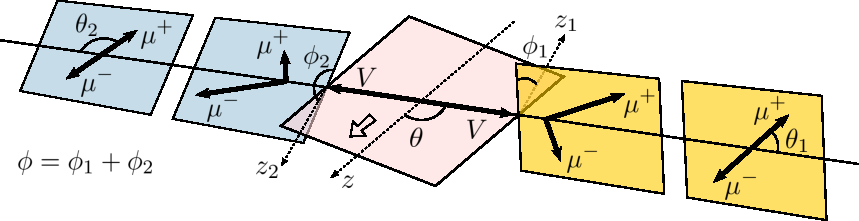
\includegraphics[width=0.8\textwidth]{../plots/angles.pdf}
  \caption{Schematic view of the $X\to V(\mu^+\mu^-)\,V(\mu^+\mu^-)$ decay kinematics.
  The black arrows shows three dimensional vectors of particles. A shaped arrow gives the direction of polarization of $X$.}
  \label{fig:X.decay}
\end{figure}
The parity leads to relation between the opposite values of helicity:
\begin{equation} \label{eq:parity}
H_{\lambda_1,\lambda_2} = P (-1)^J H_{-\lambda_1,-\lambda_2},
\end{equation}
where $P$ is internal parity of the decaying particle. The product $P (-1)^J$ is commonly referred to as the naturality.
It determines the symmetry of the matrix under reflection through the center.
Identity of the decay particle gives a relation of the helicity matrix with the transposed one.
\begin{equation} \label{eq:permutation}
H_{\lambda_1,\lambda_2} = (-1)^J H_{\lambda_2,\lambda_1},
\end{equation}
The matrices of the helicity couplings are symmetric (anti-symmetric) for the even-spin (odd-spin) decay particle.
Combining two symmetries we split all possible quantum numbers $J^P$ into four groups as shown in Tab.~\ref{tab:couplings}.
\begin{table}
  \caption{Possible quantum numbers of the decaying particle $X$ separated to four groups with respect of symmetry of the helicity matrix. The framed quantum numbers in the last column have additional restrictions due to the maximal value of the spin projection.}
  \label{tab:couplings}
  \begin{tabular}{c | r | r | l}
    group & $(-1)^{J}$ & $P(-1)^{J}$ & explicit $J^P$\\\hline
    \I    & even($+$) &   natural($+$) & \fbox{$0^+$}, $2^+$, $4^+$, $6^+$\\
    \II   & even($+$) & unnatural($-$) & \fbox{$0^-$}, $2^-$, $4^-$, $6^-$\\
    \III  & odd($-$)  &   natural($+$) &        $1^-$, $3^-$, $5^-$, $7^-$\\
    \IV   & odd($-$)  & unnatural($-$) & \fbox{$1^+$}, $3^+$, $5^+$, $7^+$
  \end{tabular}
\end{table}
The relations Eq.~\eqref{eq:parity} and Eq.~\eqref{eq:permutation} greatly reduce the number of free components of the helicity matrix.
\begin{align}
  H_\I&=\begin{pmatrix}
    b & a & c\\
    a & d & a\\
    c & a & b
  \end{pmatrix}_S&
  H_\II&=\begin{pmatrix}
    b & a &  \\
    a &   & -a\\
      & -a & -b
  \end{pmatrix}_S&
  H_{\III}&=\begin{pmatrix}
      & a &  \\
    -a &   & -a\\
      & a &
  \end{pmatrix}_A&
  H_{\IV}&=\begin{pmatrix}
      & a & c\\
    -a &   & a\\
    -c & -a &
  \end{pmatrix}_A
\end{align}
There are three special cases, $0^+$ of the first group for which $a=c=0$,
$0^-$ in the second group with $a=0$, and $1^+$ in the forth group with $c=0$.
% \begin{align} \label{eq:matrices.spec}
%   H_\I^{(0^+)}&=\begin{pmatrix}
%     b & & \\
%     & d &\\
%     & & b
%   \end{pmatrix}_S&
%   H_\II^{(0^-)}&=\begin{pmatrix}
%     b &  &  \\
%      &   & \\
%       &  & -b
%   \end{pmatrix}_S&
%   H_{\IV}^{(1^+)}&=\begin{pmatrix}
%       & a & \\
%     -a &   & a\\
%       & -a &
%   \end{pmatrix}_A
% \end{align}


\section{Unpolarized decay}
The prompt production is known to yield negligible polarization \cite{Lambda@ATLAS, Charmoniub, Lambdab}. The dependence on $\theta$ disappear in that case:
\begin{equation} \label{eq:delta}
  \sum_M d_{M,\lambda_1-\lambda_2}^{J}(\theta) d_{M,\lambda_1'-\lambda_2'}^{J}(\theta) = \delta_{\lambda_1-\lambda_2,\lambda_1'-\lambda_2'}.
\end{equation}
On contrast, the observed non-trivial dependence of the intensity on $\cos\theta$
would indicate polarization of the initial state.
Once the orientation of the production plane is averaged, the intensity becomes a function of just three quantities: polar decay angles of leptons, the difference on the azimuthal angles, $\phi = \phi_1+\phi_2$. It is easy to see transforming the azimuthal dependence,
\begin{equation}
i\lambda_1\phi_1+i\lambda_2\phi_2 = i(\lambda_1-\lambda_2)\phi_1+i\lambda_2\phi
\end{equation}
The first term on the left side of the expression vanishes once the amplitude is multiplied
to the conjugated with help of Eq.~\eqref{eq:delta}.

\section{Test statistics}
The most powerful method for testing spin hypothesis is the multidimensional fit.
For simplicity we consider the case of the negligible polarization in three dimensions, while all discussion is easy to generalize to the five dimensional case that includes
the polarization degrees of freedom.
The test statistics is defined by
\begin{align}
  \TS_{M/M'} = \LLH_M - \LLH_{M'},
\end{align},
where the $\LLH_M$ is the maximized value of the log likelihood over the set of helicity couplings.
\begin{equation}
  \LLH_M = \frac{1}{N_\mathrm{ev}} \sum_{e=1}^{N_\mathrm{ev}} \log I(\tau_e|M\{\hat{h}\}).
\end{equation}
The intensity $I(\tau_e|\hat{c})$ is calculated for the kinematic variables of the event $e$.
The optimized model parameters are demoted by $\hat{h}$.

Normalization for the fitted density is established using the relation,
\begin{align}
  \int I(\theta_1,\theta_2,\phi)\,\frac{\diff\cos\theta_1\,\diff\cos\theta_2\,\diff \phi}{8\pi} = N \sum_{\lambda_1,\lambda_2} |H_{\lambda_1\lambda_2}|^2.
\end{align}

Fig.~\ref{fig:TS.fixedH} shows an example of the test-statistics distribution obtained on the statistical sample of the fixed group-\III coupling matrix.

\begin{figure}
  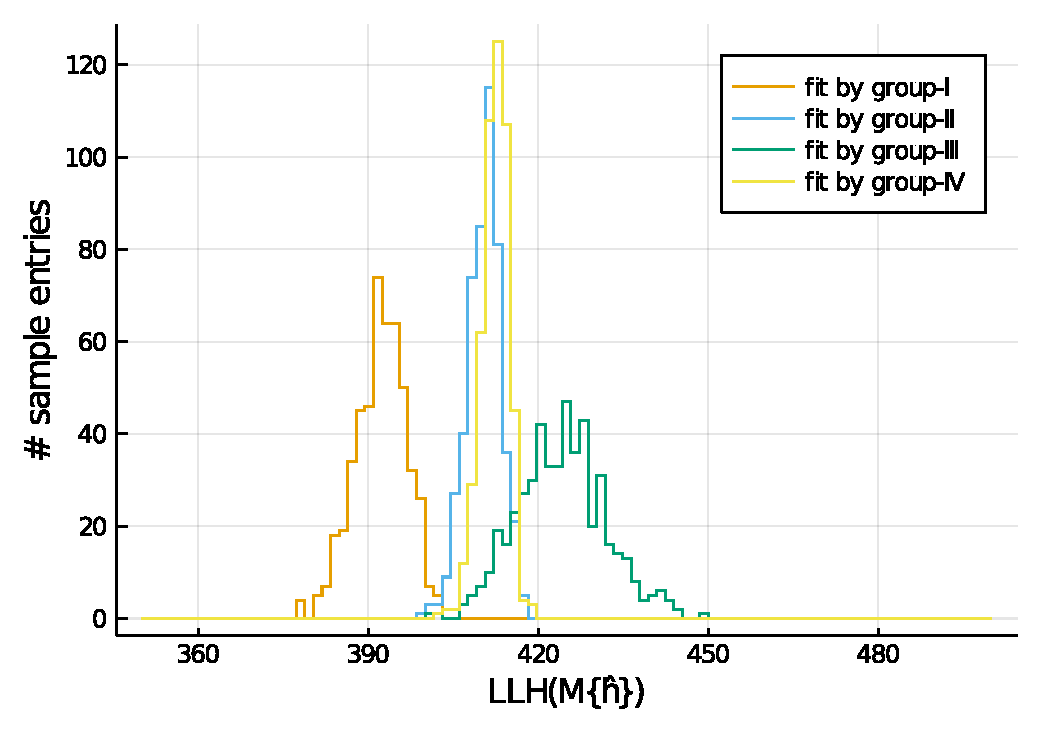
\includegraphics[width=0.48\textwidth]{../plots/llh_testing_higgs.pdf}
  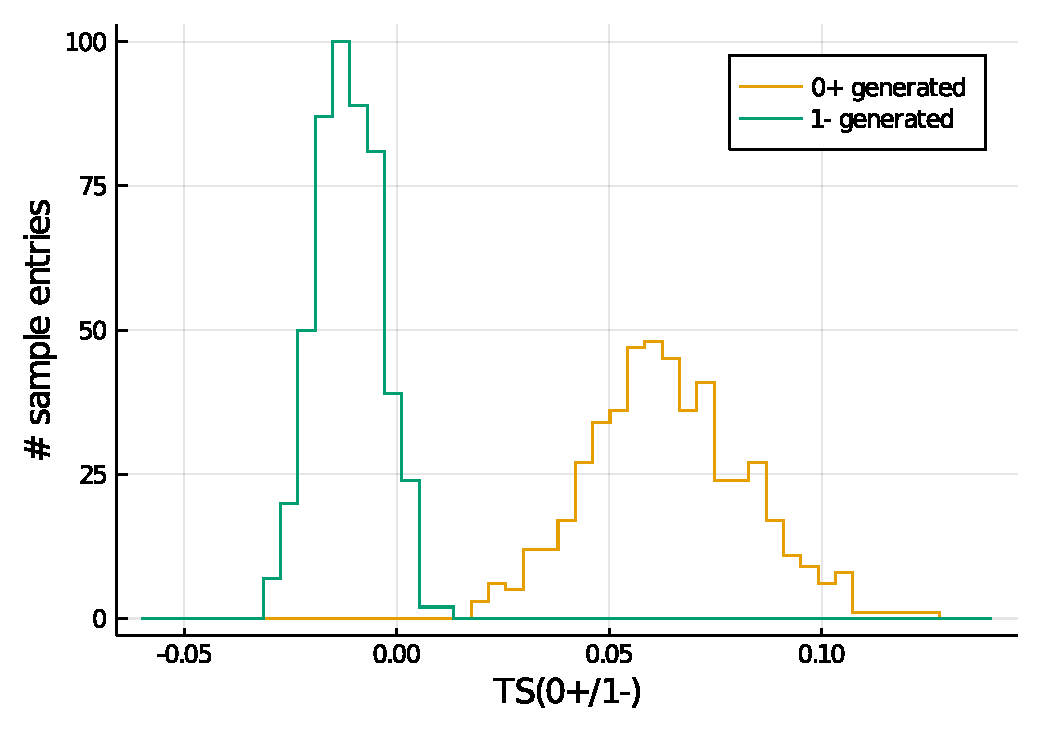
\includegraphics[width=0.48\textwidth]{../plots/TS_0p_vs_1m.pdf}
  \caption{Test statistics distribution testing hypothesis of groups $\I-\IV$ and the special cases on the statistical ensemble of the $500$ events data samples generated based on
  the fixed group-$\III$ coupling matrix. }
  \label{fig:TS.fixedH}
\end{figure}

\section{Spin of the Higgs-boson}
The most famous particle decaying to two identical vectors is the Higgs boson.
In order to validate out approach we performed analysis of the reaction $H\to Z(\mu^+\mu^-)Z(e^+e^-)$.
% A sample of $500$ events was generated using the MadGraph.
The interaction vertex of Higgs with a pair of $Z^0$ bosons is $2i m_Z^2/v\,g^{\mu\nu}$,
hence the helicity amplitude reads:
\begin{equation} \label{eq:HZZ}
  A^{H\to ZZ}_{\lambda_1,\lambda_2} = 2i\frac{m_Z^2}{v} (\epsilon_1^*(\lambda_1)\cdot\epsilon_2^*(\lambda_2)).
\end{equation}
Using the explicit expressions for the polarization $\epsilon$ vectors,
we find a special case of the matrix for group-$\I$,
\begin{equation}
  H \sim \begin{pmatrix}
    1 & &\\
    & 1+\frac{2p^2}{m^2} &\\
    & & 1
\end{pmatrix}
\end{equation}
The matrix is proportional to identity (S-wave) close to the nominal $ZZ$ production threshold,
the contribution of the $D$-wave is given by $p^2/m^2$.
 % is proportional to identity close to the production threshold, $, i.e. $b=d=1/\sqrt{3}$ in .

% The Standard Model on the tree level predicts a simple coupling of the Higgs to a pair of $Z^0$ bosons.
% \begin{equation}
%   \mathcal{L}_{HZZ} = \frac{1}{2}m_Z^2 Z^\mu Z_\mu \frac{}{})
% \end{equation}

\section{How the fit distinguishes hypothesis}

Distribution over $\phi$ angle once $\theta_1$ are $\theta_2$ are integrated:
\begin{align}
  \frac{2\pi}{N}\frac{\diff N}{\diff \phi} = 1
   + \frac{h_{1,1} h_{-1,-1}^*}{2} \cos(2 \phi),
\end{align}
The sign of the $\cos(2\phi)$ component depends on $J^P$: it is positive for quantum numbers of the first group, and negative for the ones in the second group.
The decays from the third and fourth groups do not show $2\phi$ dependence.
This sing can be determined by either fitting $\phi$ spectra, or calculating $\cos(2\phi)$ moment,
\begin{equation}
  M_{\cos(2\phi)} = \frac{1}{N_D}\sum_{e=1}^{N_D} \cos(2\phi_e).
\end{equation}

Useful relations for $\cos\theta$ integrals
\begin{align}
  3 \sum_{\xi}^{\{-1,1\}} \int_{-1}^{1} \diff \cos\,\theta d_{\lambda,\xi}^{1}(\theta) d_{\lambda',\xi}^{1}(\theta) =
  \begin{pmatrix}2 & 0 & 1\\0 & 2 & 0\\1 & 0 & 2\end{pmatrix}_{\lambda\lambda'},\\
  %
  % 3 \sum_{\xi}^{\{-1,1\}} \int_{0}^{1} \diff \cos\,\theta d_{\lambda,\xi}^{1}(\theta) d_{\lambda',\xi}^{1}(\theta) =
  % \frac{1}{2}\begin{pmatrix}2 & -\frac{1}{\sqrt{2}} & 1\\-\frac{1}{\sqrt{2}} & 2 & \frac{1}{\sqrt{2}}\\1 & \frac{1}{\sqrt{2}} & 2\end{pmatrix}_{\lambda\lambda'},\\
  %
  3 \int_{-1}^{1} \diff \cos\,\theta d_{\lambda,0}^{1}(\theta) d_{\lambda',0}^{1}(\theta) =
  \begin{pmatrix}1 & 0 & -1\\0 & 1 & 0\\-1 & 0 & 1\end{pmatrix}_{\lambda\lambda'},\\
\end{align}

\begin{figure}
  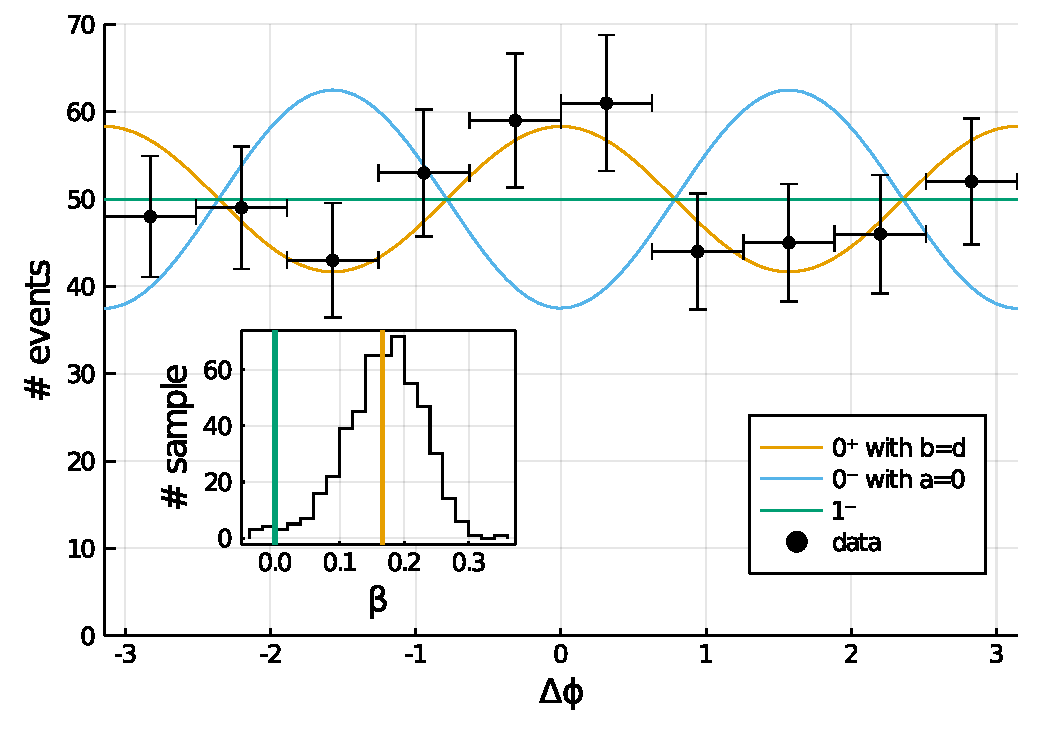
\includegraphics[width=0.48\textwidth]{../plots/phi_higgs.pdf}
  \caption{}
  \label{}
\end{figure}

\section*{Acknowledgement}
The project was motivated by discussion in the LHCb Amplitude Analysis group.
Especially we thank Biplab Day for organizing seminar dedicated to $X\to VV$.
We gratefully acknowledge Alessandro Pilloni for useful comments on the work.
We thank Liupan An and Ronan McNulty for finding practical cases for the analysis.

\appendix

\section{Polarization vectors}

For calculation of the Higgs decay ampluitude in Eq.~\eqref{eq:HZZ}
we used explicit expressions for the polarization vectors:
\begin{align}
  \epsilon_z^{\mu}(\pm1) &= \frac{1}{\sqrt{2}} \left( 0,\mp 1,-i,0 \right), &
  \epsilon_z^{\mu}(0) &= \frac{1}{m_Z} \left(p,0,0,E\right),
\end{align}
where $E$, $p$, and $m_Z$ are the energy, momentum, and the mass of the $Z$ boson.
The general expressions for the rotational vectors follows:
\begin{align}
  % \epsilon_1(\pm1) &= R_z(\phi) R_y(\theta) (0,-i,\mp 1,0)\frac{1}{\sqrt{2}},\\
  % \epsilon_2(\pm1) &= R_z(\phi) R_y(\theta) R_y(\pi) (0,-i,\mp 1,0)\frac{1}{\sqrt{2}};\\
  % \epsilon_1(0) &= R_z(\phi) R_y(\theta) (-p,0,0,E)\frac{1}{m},\\
  % \epsilon_2(0) &= (-1) R_z(\phi) R_y(\theta) R_y(\pi) (-p,0,0,E)\frac{1}{m},
  \epsilon_1(\lambda) &= R_z(\phi) R_y(\theta) \epsilon_z(\lambda),\\
  \epsilon_2(\lambda) &= (-1)^{1-\lambda} R_z(\phi) R_y(\theta) R_y(\pi) \epsilon_z(\lambda),\\
\end{align}
where $R_y(\phi)R_y(\theta)$ is a product of the three-dimensional rotation matrices
that transforms the vector $(0,0,1)$ to the direction $(\sin\theta\cos\phi,\,\sin\theta\sin\phi,\,\cos\theta)$.
The particle-2 requires additional rotation by $\pi$ about the $y$ axis. We also use the particle-two phase convention,
$(-1)^{1-\lambda_2}$ that adds an extra sign to the vector $\epsilon_2(0)$.

\section{$\eta s$ invariance}

\begin{equation}
  H = \begin{pmatrix}
    0 &1 &0 \\
    s & 0 &s\eta \\
    0 &\eta &0
  \end{pmatrix}
\end{equation}
The intensity reads:
\begin{align}
  I(H) &= \frac{s^{2} \eta^{2} \sin^{2}{\left (\theta_{1} \right )} \cos^{2}{\left (\theta_{2} \right )}}{2} + \frac{s^{2} \eta^{2} \sin^{2}{\left (\theta_{1} \right )}}{2} + \frac{s^{2} \sin^{2}{\left (\theta_{1} \right )} \cos^{2}{\left (\theta_{2} \right )}}{2} + \frac{s^{2} \sin^{2}{\left (\theta_{1} \right )}}{2} \\ \nonumber
   &\quad + \frac{s \eta \left(\cos{\left (- 2 \theta_{1} + 2 \theta_{2} + \phi \right )} + \cos{\left (2 \theta_{1} - 2 \theta_{2} + \phi \right )} - \cos{\left (2 \theta_{1} + 2 \theta_{2} - \phi \right )} - \cos{\left (2 \theta_{1} + 2 \theta_{2} + \phi \right )}\right)}{8}\\ \nonumber
   &\quad+\frac{\eta^{2} \sin^{2}{\left (\theta_{2} \right )} \cos^{2}{\left (\theta_{1} \right )}}{2} + \frac{\eta^{2} \sin^{2}{\left (\theta_{2} \right )}}{2} + \frac{\sin^{2}{\left (\theta_{2} \right )} \cos^{2}{\left (\theta_{1} \right )}}{2} + \frac{\sin^{2}{\left (\theta_{2} \right )}}{2}
\end{align}
The expression does not change under flip of $\eta$ and $s$ sign simultaneously.
Hence the group-$\III$ cannot be distinguished from the group-$\II$.

\bibliography{ref}
\end{document}




% \begin{align}
%   \frac{\diff^2 N}{\diff \cos\theta_1\,\diff \cos\theta_2} =
%   |H_{\lambda_1\lambda_2}|^2
%   \sum_{\xi_1,\xi_2}^{\{-1,1\}}
%   9|d_{\lambda_1,\xi_1}^{1}(\theta_1) d_{\lambda_2,\xi_2}^{1}(\theta_2)|^2.
% \end{align}

% \section{LS couplings}
%
% \begin{align}
%   H_{\lambda_1,\lambda_2} = (-1)^{j_2-\lambda_2} \sum_{ls} \sqrt{\frac{2l+1}{2j+1}}
%   \left\langle 1,\lambda_1;1,\lambda_2|s,\lambda_1-\lambda_2 \right\rangle
%   \left\langle L,0;s,\lambda_1-\lambda_2|j,\lambda_1-\lambda_2 \right\rangle H_{ls}.
% \end{align}
%
% \begin{align*}
%   1^-\otimes 1^-: && S:\qquad & {\color{cola} 0^+}\quad {\color{colb} 1^+}\quad {\color{colc} 2^+},\\
%                   && P:\qquad & \color{gray} 1^-\quad (0^-,1^-,2^-)\quad (1^-,2^-,3^-),\\
%                   && D:\qquad & {\color{colc} 2^+}\quad ({\color{colb} 1^+},{\color{colc} 2^+},3^+)\quad ({\color{cola} 0^+},{\color{colb} 1^+},{\color{colc} 2^+},3^+,4^+),\\
%                   && F:\qquad & \color{gray} 3^-\quad (2^-,3^-,4^-)\quad (0^-,1^-,2^-,3^-,4^-),\\
%                   && H:\qquad & 4^+\quad (3^+,4^+,5^+)\quad ({\color{colc} 2^+},3^+,4^+,5^+,6^+).
% \end{align*}

% \section{Odd and even spins}

% \begin{figure}
%   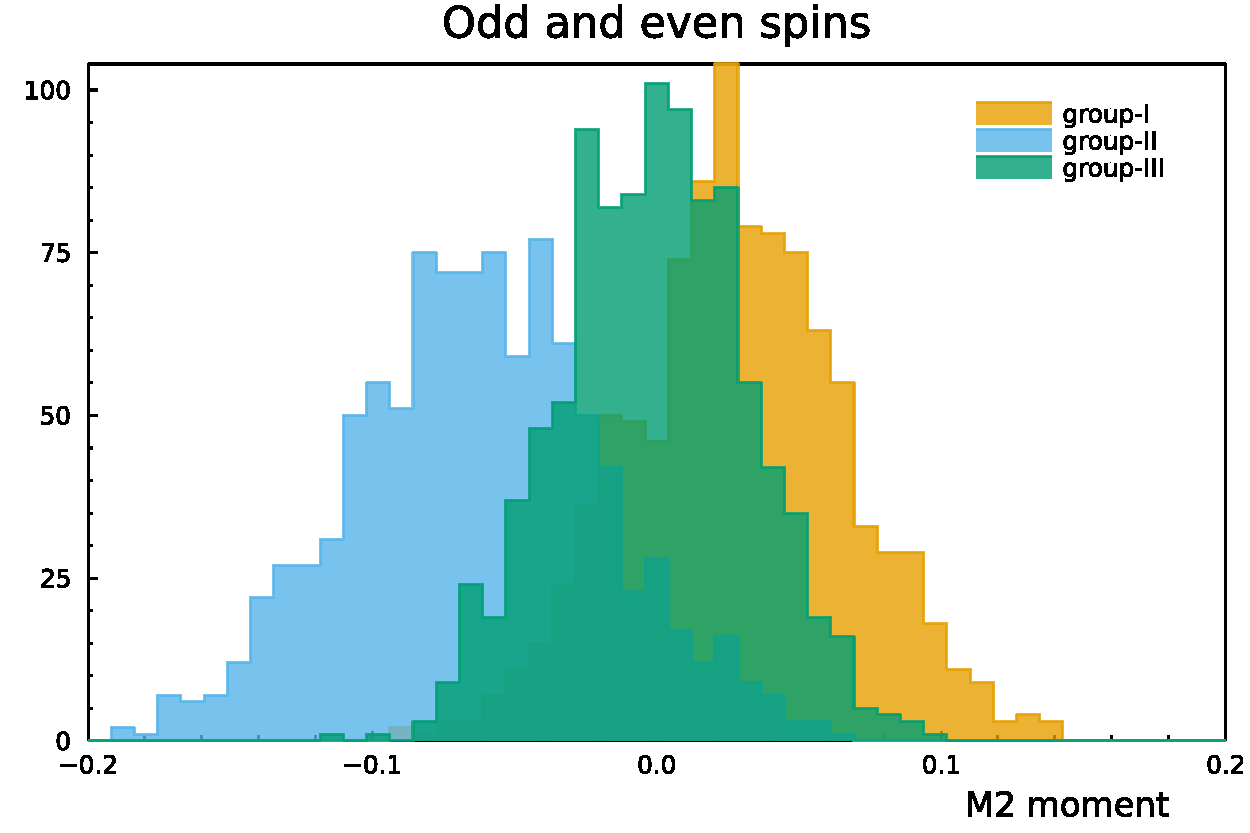
\includegraphics[width=0.46\textwidth]{../plots/moment_M2phi_Nev=500.pdf}
%   \caption{Distribution of $M_{\cos(2\phi)}$ for a sample of random coupling constants.
%   A sample of $500$ events is generated for every hypothesis of couplings.}
%   \label{}
% \end{figure}
%
% \begin{figure}
%   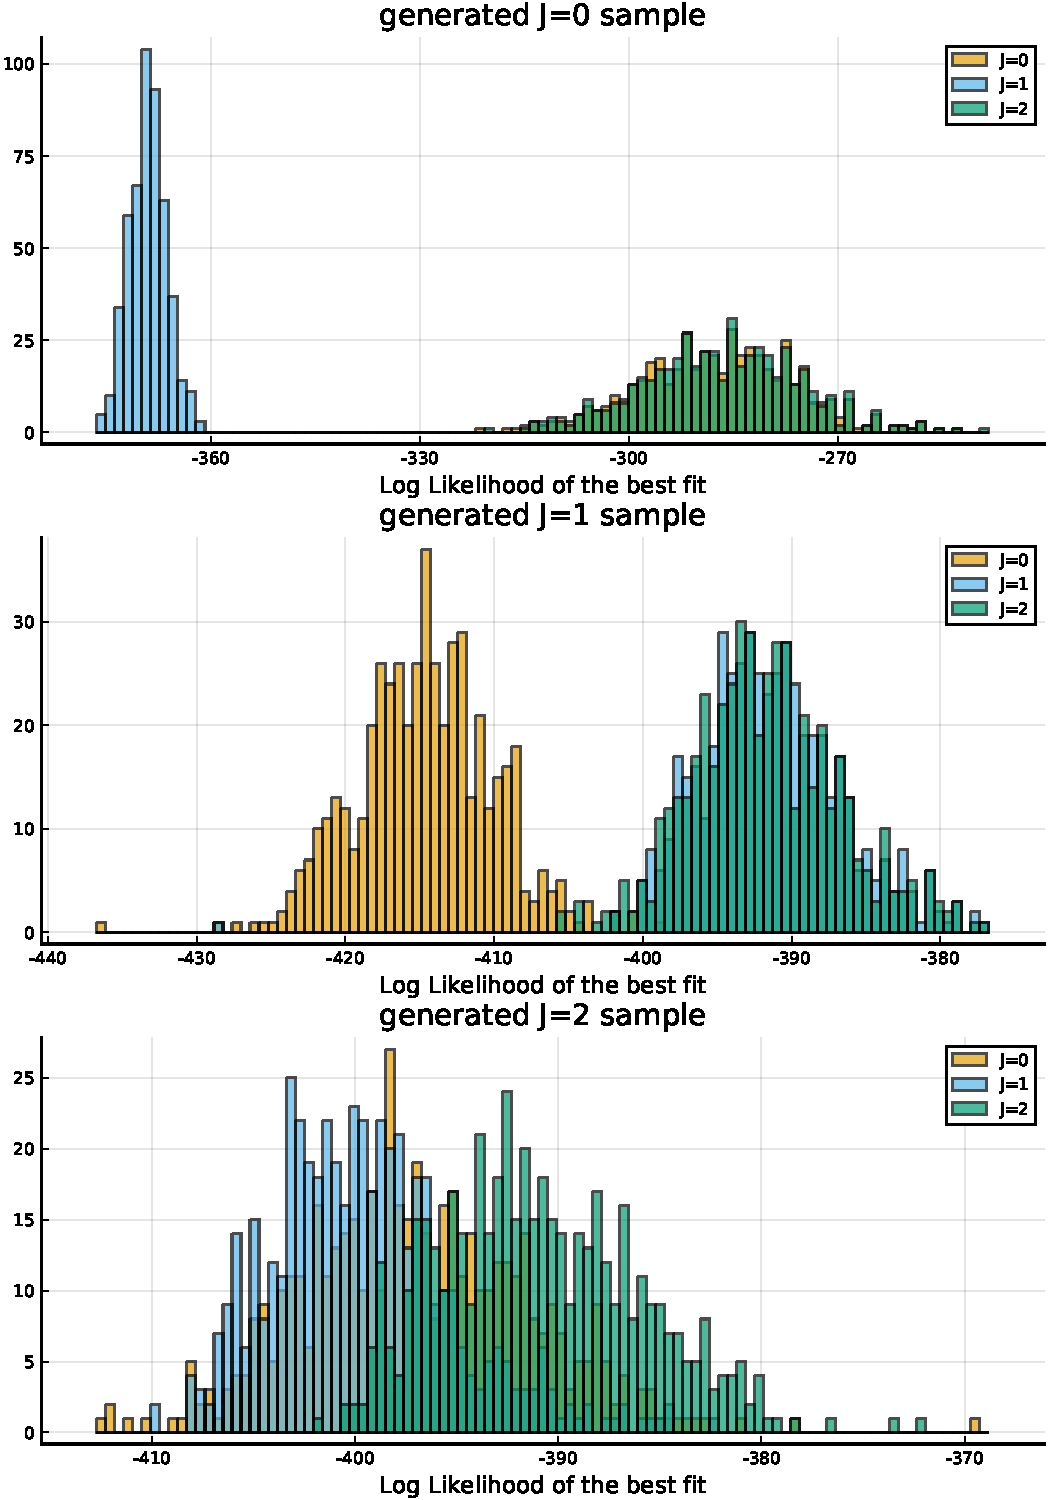
\includegraphics[width=0.9\textwidth]{../plots/llh_of_fit_of_J012.pdf}
%   \caption{Hypothesis testing with $500$ events}
%   \label{fig.3dfit}
% \end{figure}


% Matrices of couplings without the phase $(-1)^{j_2-\lambda_2}$ are symmetric (round brackets) or asymmetric (square parentheses)
% \begin{itemize}
%   \item $j = 0$:
% \begin{align*}
%   % l = 0, s = 0
%   \frac{\sqrt{3}}{3}
%   \begin{pmatrix}1 & 0 & 0\\0 & -1 & 0\\0 & 0 & 1\end{pmatrix}&&
%   % l = 2, s = 2
%   \frac{\sqrt{6}}{6}
%   \begin{pmatrix}1 & 0 & 0\\0 & 2 & 0\\0 & 0 & 1\end{pmatrix}
% \end{align*}
%   \item $j = 1$:
% \begin{align*}
%   % l = 0, s = 1
%   \frac{\sqrt{6}}{6}
%   \begin{pmatrix}-1 & -1 & 0\\-1 & 0 & 1\\0 & 1 & 1\end{pmatrix}&&
%   % l = 2, s = 1
%   \frac{\sqrt{3}}{6}
%   \begin{pmatrix}2 & -1 & 0\\-1 & 0 & 1\\0 & 1 & -2\end{pmatrix}&&
%   % l = 2, s = 2
%   \frac{1}{2}
%   \left[\begin{matrix}0 & -1 & 0\\1 & 0 & -1\\0 & 1 & 0\end{matrix}\right]
% \end{align*}
% \item $j = 2$:
% \begin{align*}
%   % l = 0, s = 2
%   \frac{\sqrt{30}}{30}
%   \begin{pmatrix}1 & \sqrt{3} & \sqrt{6}\\\sqrt{3} & 2 & \sqrt{3}\\\sqrt{6} & \sqrt{3} & 1\end{pmatrix}&&
%   % l = 2, s = 0
%   \frac{\sqrt{3}}{3}
%   \begin{pmatrix}1 & 0 & 0\\0 & -1 & 0\\0 & 0 & 1\end{pmatrix}&&
%   % l = 2, s = 1
%   \frac{1}{2}
%   \left[\begin{matrix}0 & -1 & 0\\1 & 0 & 1\\0 & -1 & 0\end{matrix}\right]&&
%   % l = 2, s = 2
%   \frac{\sqrt{7}}{14}
%   \begin{pmatrix}- \frac{2 \sqrt{3}}{3} & -1 & 2 \sqrt{2}\\-1 & -\frac{4 \sqrt{3}}{3} & -1\\2 \sqrt{2} & -1 & - \frac{2 \sqrt{3}}{3}\end{pmatrix}&&
%   % l = 4, s = 2
%   \frac{\sqrt{70}}{70}
%   \begin{pmatrix}\sqrt{6} & -2 \sqrt{2} & 1\\- 2 \sqrt{2} & 2\sqrt{6} & - 2 \sqrt{2}\\1 & -2\sqrt{2} & \sqrt{6}\end{pmatrix}
% \end{align*}
% \end{itemize}
%
% \begin{figure}
%   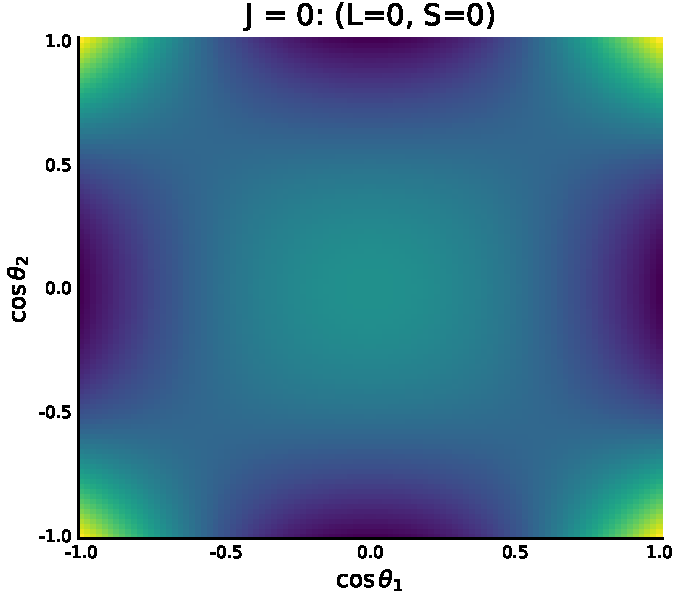
\includegraphics[width=0.195\textwidth]{../plots/map_JLS_000.pdf}
%   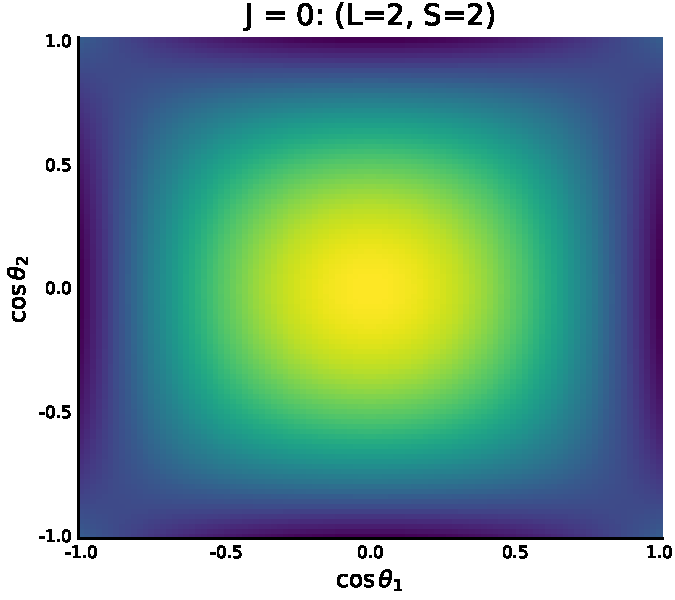
\includegraphics[width=0.195\textwidth]{../plots/map_JLS_022.pdf}
%   \caption{}
%   \label{fig.j0}
% \end{figure}
% \begin{figure}
%   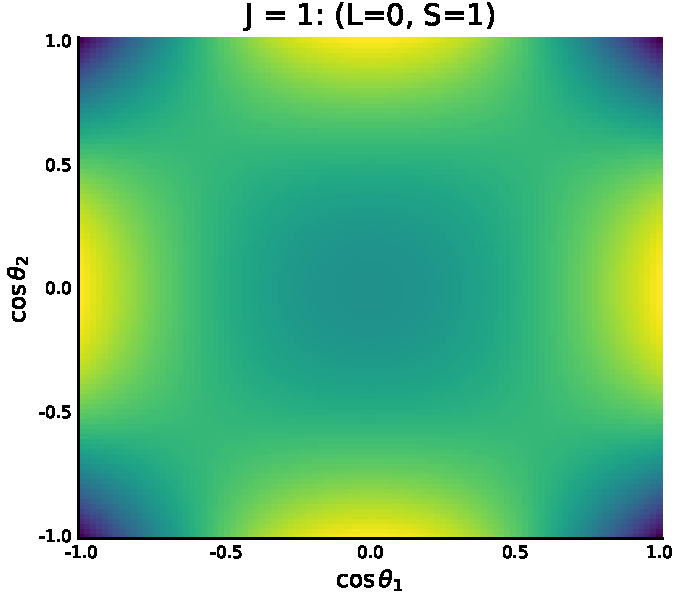
\includegraphics[width=0.195\textwidth]{../plots/map_JLS_101.pdf}
%   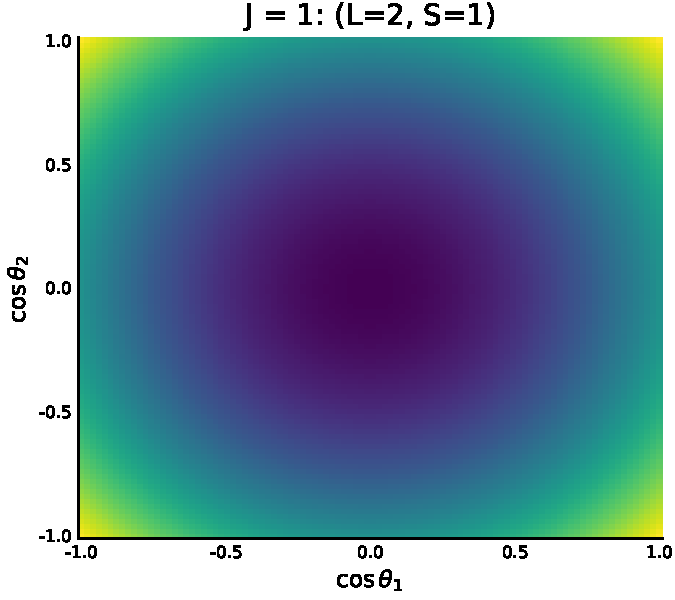
\includegraphics[width=0.195\textwidth]{../plots/map_JLS_121.pdf}
%   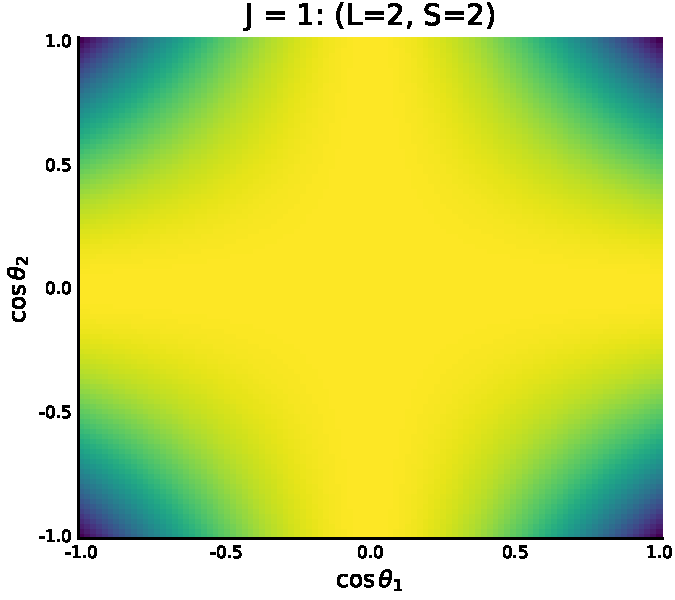
\includegraphics[width=0.195\textwidth]{../plots/map_JLS_122.pdf}
%   \caption{}
%   \label{fig.j1}
% \end{figure}
% \begin{figure}
%   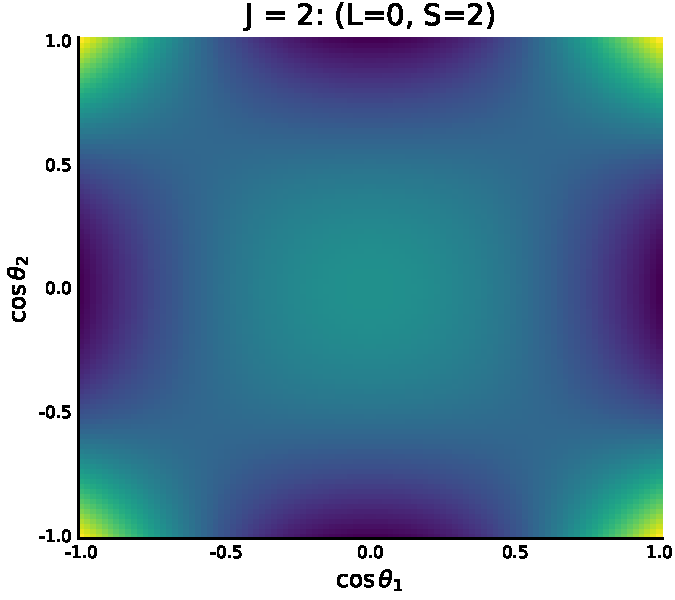
\includegraphics[width=0.195\textwidth]{../plots/map_JLS_202.pdf}
%   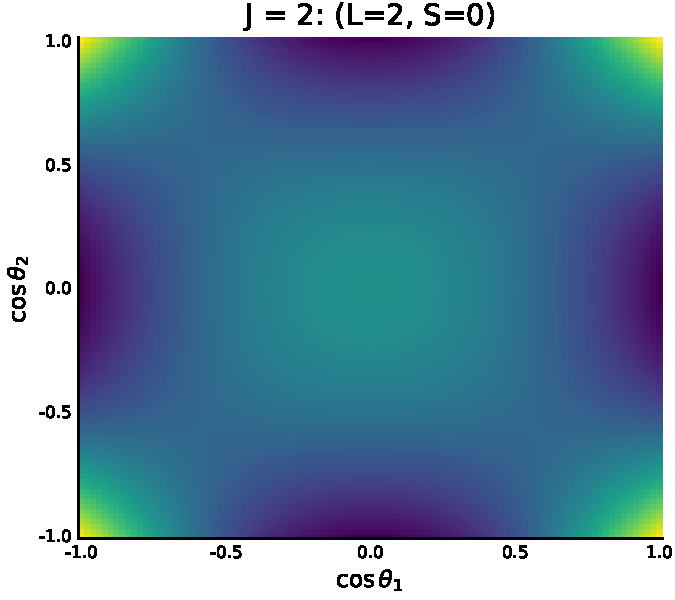
\includegraphics[width=0.195\textwidth]{../plots/map_JLS_220.pdf}
%   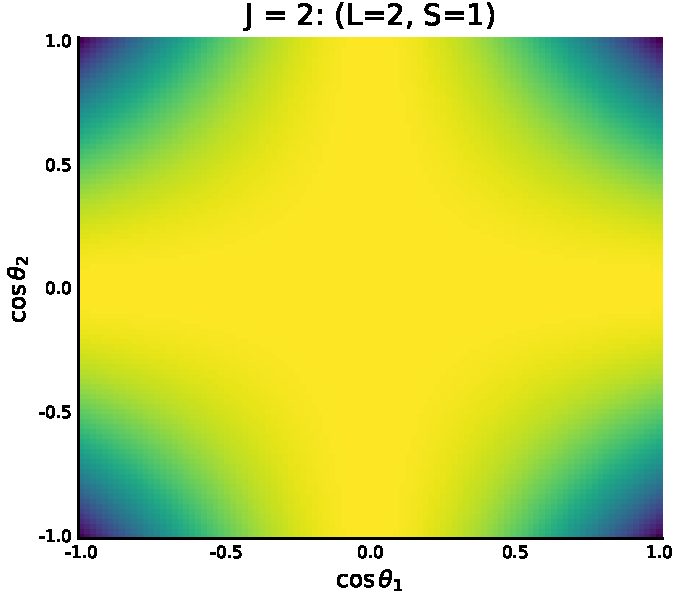
\includegraphics[width=0.195\textwidth]{../plots/map_JLS_221.pdf}
%   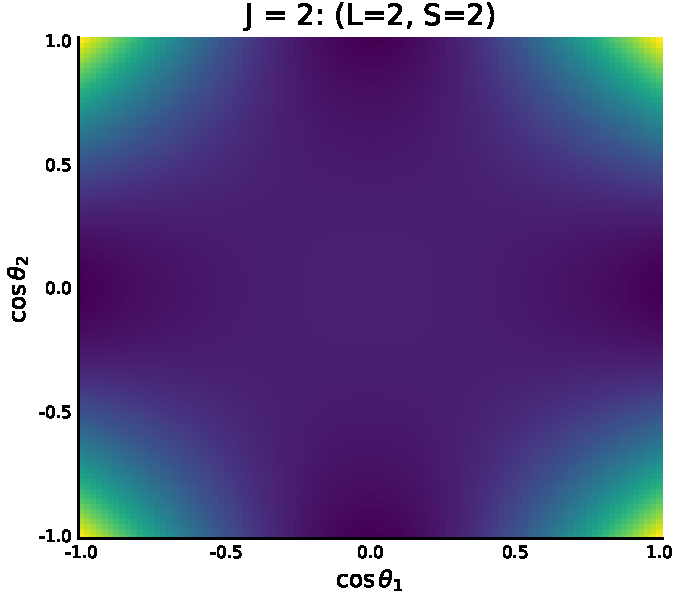
\includegraphics[width=0.195\textwidth]{../plots/map_JLS_222.pdf}
%   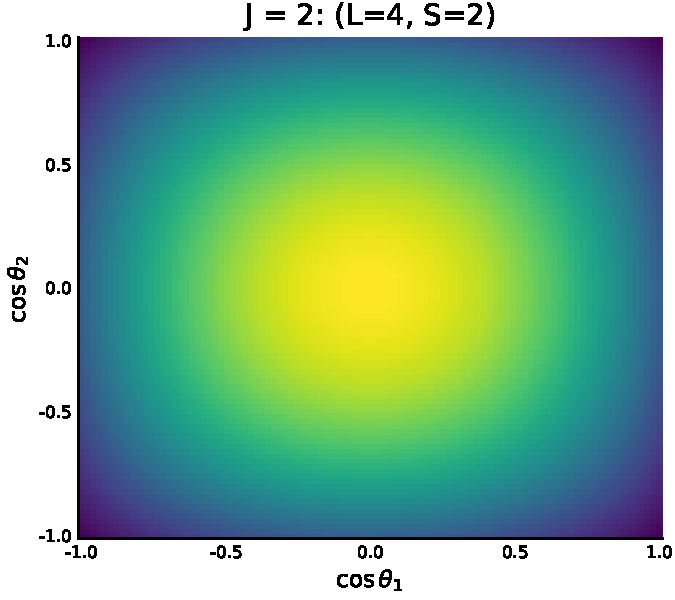
\includegraphics[width=0.195\textwidth]{../plots/map_JLS_242.pdf}
%   \caption{}
%   \label{fig.j2}
% \end{figure}


% \begin{align}
%     I(\cos\theta_1,\phi_1,\cos\theta_2,\phi_2) &= 9\sum_{M}P_M
%     \sum_{\lambda_1,\lambda_2}\sum_{\lambda_1',\lambda_2'}
%     d_{M,\lambda_1-\lambda_2}^{J}(\theta) (-1)^{1-\lambda_2}
%     d_{M,\lambda_1'-\lambda_2'}^{J}(\theta) (-1)^{1-\lambda_2'}
%     \\ \nonumber
%     &\qquad\times
%     H_{\lambda_1\lambda_2} H_{\lambda_1'\lambda_2'}^{*}
%     e^{i(\lambda_1'-\lambda_1)\phi_1}
%     e^{i(\lambda_2'-\lambda_2)\phi_2}
%     \\ \nonumber
%     &\qquad\times
%     \sum_{\xi_1}^{\{-1,1\}}
%     d_{\lambda_1,\xi_1}^{1}(\theta_1) d_{\lambda_1',\xi_1}^{1}(\theta_1)
%     \sum_{\xi_2}^{\{-1,1\}}
%     d_{\lambda_2,\xi_2}^{1}(\theta_2) d_{\lambda_2',\xi_2}^{1}(\theta_2).
% \end{align}
